%% ISAE-SUPAERO report template for research projects 
%% V1.0
%% 2016/04/14
%% by Damien Roque
%% See http://personnel.isae.fr/damien-roque


%% This template is based on bare_conf.tex
%% V1.4b
%% 2015/08/26
%% by Michael Shell

%%*************************************************************************
%% Legal Notice:
%% This code is offered as-is without any warranty either expressed or
%% implied; without even the implied warranty of MERCHANTABILITY or
%% FITNESS FOR A PARTICULAR PURPOSE! 
%% User assumes all risk.
%% In no event shall the IEEE or any contributor to this code be liable for
%% any damages or losses, including, but not limited to, incidental,
%% consequential, or any other damages, resulting from the use or misuse
%% of any information contained here.
%%
%% All comments are the opinions of their respective authors and are not
%% necessarily endorsed by the IEEE.
%%
%% This work is distributed under the LaTeX Project Public License (LPPL)
%% ( http://www.latex-project.org/ ) version 1.3, and may be freely used,
%% distributed and modified. A copy of the LPPL, version 1.3, is included
%% in the base LaTeX documentation of all distributions of LaTeX released
%% 2003/12/01 or later.
%% Retain all contribution notices and credits.
%% ** Modified files should be clearly indicated as such, including  **
%% ** renaming them and changing author support contact information. **
%%*************************************************************************

\documentclass[conference]{IEEEtran}

\usepackage[utf8]{inputenc}
\usepackage{ifthen}
\usepackage[backend=biber, style=ieee]{biblatex}
\addbibresource{references.bib}
\usepackage{hyperref}
\usepackage{url}
\usepackage[pdftex]{graphicx}
\graphicspath{{images/}}
\usepackage{tikz,filecontents}
\usetikzlibrary{shapes,arrows,shadings,patterns}
\usepackage{pgfplots}
\pgfplotsset{compat=newest}
\pgfplotsset{plot coordinates/math parser=false}
\newlength\figureheight
\newlength\figurewidth

\usepackage{amsfonts}
\usepackage[cmex10]{amsmath}
\usepackage{multirow}
\usepackage[acronym,indexonlyfirst,nomain]{glossaries}

% Examples of several macros
\newcommand*{\SET}[1]{\ensuremath{\boldsymbol{#1}}}
\newcommand*{\VEC}[1]{\ensuremath{\boldsymbol{\mathrm{#1}}}}
\newcommand*{\FAM}[1]{\ensuremath{\mathrm{#1}}}
\newcommand*{\MAT}[1]{\ensuremath{\boldsymbol{\mathrm{#1}}}}
\newcommand*{\OP}[1]{\ensuremath{\mathrm{#1}}}
\newcommand*{\NORM}[1]{\ensuremath{\left\|#1\right\|}}
\newcommand*{\DPR}[2]{\ensuremath{\left \langle #1,#2 \right \rangle}}

\newtheorem{theorem}{Theorem}

\newcommand{\alert}[1]{\textcolor{red}{#1}}
\usepackage[caption=false,font=footnotesize]{subfig}

% correct bad hyphenation here
\hyphenation{op-tical net-works semi-conduc-tor}


\begin{document}
%
% paper title
% Titles are generally capitalized except for words such as a, an, and, as,
% at, but, by, for, in, nor, of, on, or, the, to and up, which are usually
% not capitalized unless they are the first or last word of the title.
% Linebreaks \\ can be used within to get better formatting as desired.
% Do not put math or special symbols in the title.
\title{REMAINING USEFUL LIFE PREDICTIONS WITH DEEP LEARNING METHODS}

% for over three affiliations, or if they all won't fit within the width
% of the page, use this alternative format:
% 
\author{\IEEEauthorblockN{Thomas Guillebot de Nerville\IEEEauthorrefmark{1},
Paul Strähle\IEEEauthorrefmark{1},
Anass Akrim\IEEEauthorrefmark{2}\IEEEauthorrefmark{3} and 
Rob Vingerhoeds\IEEEauthorrefmark{2}}

\IEEEauthorblockA{\IEEEauthorrefmark{1}Institut Supérieur de l'Aéronautique et de l'Espace (ISAE-SUPAERO), Université de Toulouse, 31400 Toulouse, FRANCE\\
Email: \{thomas.guillebot-de-nerville,paul.strahle\}@student.isae-supaero.fr}
\IEEEauthorblockA{\IEEEauthorrefmark{2}Institut Supérieur de l'Aéronautique et de l'Espace (ISAE-SUPAERO), Université de Toulouse, 31400 Toulouse, FRANCE\\
Email: \{anass.akrim,rob.vingerhoeds\}@isae-supaero.fr}
\IEEEauthorblockA{\IEEEauthorrefmark{3}Institut Clément Ader (UMR CNRS 5312) INSA/UPS/ISAE/Mines Albi, Université de Toulouse, 31400 Toulouse, FRANCE\\
Email: anass.akrim@univ-tlse3.fr}
}


\IEEEspecialpapernotice{(Bibliography report)}
%\IEEEspecialpapernotice{(Final report)}

% import the acronyms
% Here are the acronyms
\newacronym{nlp}{NLP}{Natural Language Processing}
\newacronym{phm}{PHM}{Prognostics and Health Management}
\newacronym{rul}{RUL}{Remaining Useful Life}
\newacronym{rnn}{RNN}{Recurrent Neural Network}
\newacronym{lstm}{LSTM}{Long short-term memory}
\newacronym{gru}{GRU}{Gated Recurrent Unit}
\newacronym{cnn}{CNN}{Convolutional Neural Network}
\newacronym{tcn}{TCN}{Temporal Convolutional Network}
\newacronym{erm}{ERM}{Elman Recurrent Network}
\newacronym{mlp}{MLP}{Machine Learning Program}
\newacronym{lrdecay)}{lrDecay)}{learning rate decay}

% make the title area
\maketitle

% As a general rule, do not put math, special symbols or citations
% in the abstract
\begin{abstract}
The abstract goes here (100 words max).
\end{abstract}

\IEEEpeerreviewmaketitle

\section{Context}
\label{sec:problem-statement}

In recent years deep learning, a subbranch of machine learning, has shown impressive results, especially in the fields of speech recognition, visual object recognition and object detection \cite{LeCun2015}. One requirement to use deep learning is the presence of sufficient amounts of data \cite{Sikorska2011}. As more data becomes available in the engineering domain there is a recent surge of interest to use deep learning in engineering \cite{Voulodimos2018}.

One of the strengths of deep learning approaches is their ability to deal with and detect complex relationships in large datasets \cite{MONTEROJIMENEZ2020539}. This strength makes their usage also interesting in the \gls{phm} domain \cite{Wu2015}. The potential of deep learning in \gls{phm} might not be fully exploited yet \cite{Akrim2021}.

\section{Problem statement}
\label{sec:problem-statement}

The problem to which the deep learning algorithms are applied in this project is the crack growth in precracked aircraft fuselage panels. The Paris-Erdogan Law \cite{Paris1963} is used to create a synthetic dataset of the crack growth to train the model. The dataset consists of strain data from virtual strain gauges placed in the area around the crack and the corresponding \gls{rul} of the fuselage panels.

The goal for this project is to develop different deep learning models for \gls{rul} prediction based on different model architectures. The developed models are optimized before a comparison between them is made. Therefore an appropriate evaluation metric must be selected.

\section{Prognostics and Health Management}
\label{sec:Prognostics-and-Health-Management}

According to \textsc{Zio} \cite{Zio2012} \gls{phm} is a field of research and application which aims at making use of past, present and future information on the environmental, operational and usage conditions of an equipment in order to detect its degradation, diagnose its faults, predict and proactively manage its failures. In the context of this project only the detection of degradation and prediction of failure are relevant.

\gls{phm} models can be divided into single and multi model approaches. Multi model approaches are a combination of different single model approaches. Single model approaches can be further divided into knowledge-based, data-driven and physics-based models. Within the data-driven models there are statistical, stochastic and machine learning models which is the category of deep learning models. \cite{MONTEROJIMENEZ2020539}

\section{Deep Learning Models}
\label{sec:deep-learning-models}

Within the available deep learning models there are two algorithms which are promising for \gls{phm}: \glspl{rnn} (\textsc{Little} \cite{Little1996} and \textsc{Hopfield}  \cite{Hopfield1982}) and \glspl{cnn} (\textsc{Lecun et al.} \cite{Lecun1998}) \cite{Akrim2021}.

The common type of deep learning model for time series prediction are \glspl{rnn} \cite{Bai2018}. Standard \glspl{rnn} have some major drawbacks (vanishing/exploding gradient problem) which limit their application \cite{Bengio1994}. \gls{lstm} networks (\textsc{Hochreiter} and \textsc{Schmidhuber}) \cite{Hochreiter1997} avoid this problem and have established themselves as one of the most used deep learning model type, especially for \gls{nlp} \cite{Wu2016}. For this reasons \glspl{lstm} will be one of the investigated \gls{rnn} approaches in this project. Another investigated \gls{rnn} approach are the \glspl{gru}. It is a simplified version of the \gls{lstm}. Due to this simplicity it is gaining in popularity in recent years \cite{Rana2016}. 

Recent results suggest that \glspl{cnn} can match or even outperform \glspl{rnn} in time series related tasks \cite{Bai2018}. The second major focus of this work are therefore \gls{cnn} models. Besides the general \gls{cnn} architectures \glspl{tcn} (\textsc{Bai et al.} \cite{Bai2018}) are investigated in this work. A \gls{tcn} is a specific \gls{cnn} architecture that tries to replicate some of the best practices for \gls{cnn} architectures. As depicted in Fig. \ref{fig:tcn-architecture} a \gls{tcn} is composed of convolutional layers which include dilation. Through dilation \glspl{tcn} can increase their receptive field and therefore capture relationships over longer time sequences. For more details on \glspl{tcn} see \cite{Bai2018}.

\begin{figure}[htp]
	\centering
	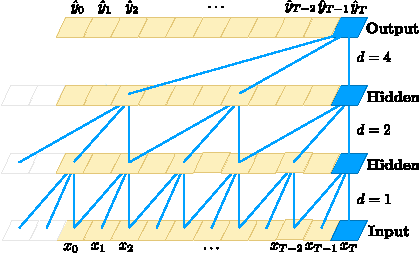
\includegraphics[width=6cm]{tcn_architecture.pdf}
	\caption{\gls{tcn} with dilation factors d = 1; 2; 4 and filter size k = 3 \cite{Bai2018}}
	\label{fig:tcn-architecture}
\end{figure}

\section{Applications of Deep Learning in Prognostics}
\label{sec:applications-of-deep-learning-in-prognostics}

\glspl{rnn} are as stated in chapter \ref{sec:deep-learning-models} the common approach for time-dependent relationships and have therefore also achieved great interest in the \gls{phm} domain \cite{Akrim2021}.

% Add citations in section below

Pioneers models were developed such as \glspl{erm} or Jordan Networks, outperforming traditional \glspl{mlp} for sequence-prediction \cite{Akrim2021}. These algorithms were then widely explored by several researchers. Among them can be cited \textsc{Yan et al.} for their work on material degradation evaluation and life prediction in 2007, and \textsc{Kramti et al.} for having used \glspl{erm} for high-speed shaft bearing prognostics based on vibration signals \cite{Akrim2021}.

The common \gls{cnn} models deal with 2-Dimensional data as input such as pictures. The time sequence data used for \gls{phm} is in 1-Dimensional format. For this application 1D-\gls{cnn} have been introduced. The key differences between them and the 2D-\glspl{cnn} are that their input data is reduced by one dimension and the convolution filter only slides in one dimension. \cite{Akrim2021}

In one of the first applications of \glspl{cnn} to \gls{phm} \textsc{Li et al.} suggested that \glspl{cnn} can be used to obtain \gls{rul} prognoses for machinery \cite{Li2018}. The model was applied to the C-MAPSS dataset \cite{Saxena2008} and outperformed state-of-the-art prognostics approaches including \gls{rnn} and \gls{lstm} models. To prepare the data for the \gls{cnn} a sliding window approach was used. This approach maps the \gls{rul} at time $ t_i $ to the current and past time steps of the input features $ [x_{t-N+1}, x_{t-N+2},..., x_{t-1}, x_t] $ where $ N $ is the length of the sequence. The resulting input matrix has therefore the dimension $ k \times N $ where $ k $ is the number of features.

% ADD MORE CNN FOR PHM EXAMPLES HERE

As it showed promising results in other applications of deep learning to \gls{phm} (\cite{Liu2019a, Xiao2016}), classification is an interesting alternative to regression for \gls{rul} prediction. Instead of trying to predict an exact \gls{rul} value the goal is to predict the correct \gls{rul} class with a lower and upper bound for the \gls{rul}.

\section{Research relevance}
\label{sec:research-relevance}

The goal of this study is to predict the \gls{rul} of precracked aircraft fuselage panels based on strain gauge measurements using deep learning. This approach is driven by the impressive results of deep learning to \gls{rul} prediction as shown in \cite{Xu2018, Li2018, Liu2019, Yuan2016, Wu2018, Park2020} and other publications (For an overview see \textsc{Akrim et al.} \cite{Akrim2021}). Strain gauges play a vital role in \gls{phm} in general \cite{Tinga2019} and specifically for the aircraft domain \cite{Timothy2009}. According to \textsc{Fink et al.} \cite{Fink2020} is the use of simulation environments and adaption to real-life applications a promising future research approach as the data will more likely be sufficient in the source domain. The synthetic dataset used for this study aims at using this advantages. For the application of deep learning to crack growth for \gls{rul} prediction based on strain gauge measurements no results in the literature could be found. This study tries to fill this research gap.


\printbibliography

\end{document}


